\documentclass[adobefonts, a4paper]{ctexart}

\usepackage[top=1.2in, bottom=1.2in, left=1in, right=1in]{geometry}
\usepackage{minted, graphicx, hyperref}

\hypersetup{colorlinks=true, linkcolor=blue}

\title{操作系统实验报告4}
\author{蔡日骏\quad12348003}

\begin{document}
\maketitle

\section{概述}
本次实验在上次实验基础上增加的通过中断实现的系统调用功能,同时对上个版本做了一些优化。

\section{基本设计}
本次实验的一个要求是在屏幕右下角实现一个能独立运行的旋转的标志。这个功能使用IRQ0(\verb|0x08|号中断)
自动触发的\verb|0x1C|号中断实现即可,非常简单,具体实现请看下节。

实验的另外两个要求是实现键盘事件的响应,以及在屏幕上显示一些信息。我这里直接实现了几个POSIX标准
的系统调用,方便以后扩展。系统调用的ABI与老版本的Linux内核一致,\verb|eax|寄存器保存功能号,
其他通用寄存器保存参数,使用\verb|0x80|号中断触发。

目前我已经实现的系统调用有\verb|_exit|、\verb|read|、\verb|write|、\verb|time|四个。其中\verb|read|
和\verb|write|目前只支持在控制台上读写。

此外,为了方便在系统调用中访问用户程序的数据,本次实验中用户程序拥有独立于内核的堆栈段,而用户程序
的堆栈段与代码段重合,这样当用户程序向系统调用传递堆栈上的空间的地址时,系统调用就不需要对其进行特殊
的处理了,只需要切换到用户程序的段即可访问,访问完成后切换回内核段中即可。

\section{具体实现}

由于GCC不支持x86平台的nacked函数,使用C语言编写的中断处理程序需要有一个汇编语言编写的Wrapper。为了
方便起见,在\verb|int_handler_wrappers.nasm|中定义了下面这个宏:

\begin{minted}{nasm}
%macro WRAP_INT_HANDLER 1
extern _%1
global %1
%1:
    call dword _%1
    iret
%endmacro
\end{minted}

同时,为了方便修改中断向量表,定义了下面的函数:

\begin{minted}{nasm}
;add_int_handler
;Add a interrupt handler into the IVT
;   0: Interrupt number
;   1: Offset of the handler (must be in the current CS)
;Returns: EAX: The original handler
add_int_handler:
    enter 0, 0
    push bx
    push ds
    xor bx, bx
    mov ds, bx
    mov bl, [bp+6]
    shl bx, 2

    mov ax, cs
    shl eax, 8
    mov ax, [bp+10]

    xchg [ds:bx], eax

    pop ds
    pop bx
    leave
    pop ecx
    jmp cx
\end{minted}

需要定义向量处理程序时,使用C语言实现以\verb|_|开头的处理函数,然后添加对应的Wrapper,
再调用\verb|add_int_handler|函数即可。例如实现屏幕右下角的旋转标志:

\begin{minted}{c}
/* int_handler_wrappers.h */
void spin_mark();

/* os.c */
int main()
{
    /* ... */
    add_int_handler(0x1c, (void *)spin_mark);
    /* ... */
}

void _spin_mark()
{
    static int8_t current = 0, acc = 3;
    const char * const marks = "|/-\\|/-\\";
    uint16_t current_cursor;
    if(!--acc) {
        current_cursor = get_cursor();
        set_char(marks[current++], 0x184f);
        move_cursor(current_cursor);
        current %= 8;
        acc = 3;
    }
}
\end{minted}

\begin{minted}{nasm}
; int_handler_wrappers.nasm
WRAP_INT_HANDLER spin_mark
\end{minted}

实现系统调用时,\verb|_syscall|函数根据功能号调用相应的系统调用实现函数\verb|sys_XXX|。
如果该系统调用尚未实现,则设置\verb|errno|为\verb|ENOSYS|。同时,这个函数中需要把数据段
设置到内核段以保证系统调用正常运行。由于目前只有4个调用,为简单起见,直接使用\verb|switch|
语句做dispatch。

\begin{minted}{c}
void _syscall()
{
    __asm__ volatile(
        ".intel_syntax noprefix;"
        "mov di, cs;"
        "mov ds, di;"
        "mov es, di;"
        ".att_syntax;"
        : : : "di"
    );

    register int32_t syscall_num asm("eax"),
                     p1          asm("ebx"),
                     p2          asm("ecx"),
                     p3          asm("edx");

    errno = 0;
    switch(syscall_num)
    {
        case 1:
            sys_exit(p1); break;
        case 3:
            syscall_num = sys_read(p1, (void *)p2, p3); break;
        case 4:
            syscall_num = sys_write(p1, (void *)p2, p3); break;
        case 13:
            syscall_num = sys_time((time_t *)p1); break;
        default:
            errno = ENOSYS;
    }
}
\end{minted}

在具体实现系统调用函数时,为了方便在内核段和用户段之间跳转,定义了下面两个宏:

\begin{verbatim}
#define USER_SPACE_START __asm__ volatile\
    (".intel_syntax noprefix;mov di, 0x7d0;mov ds, di;.att_syntax;":::"di")
#define USER_SPACE_END __asm__ volatile\
    (".intel_syntax noprefix;xor di, di;mov ds, di;.att_syntax;":::"di")
\end{verbatim}

在需要访问用户程序段中的数据时,使用\verb|USER_SPACE_START|和\verb|USER_SPACE_END|
包围起相关代码即可。比如下面的代码把\verb|buf|指向的位于用户程度段中的数据写到控制台中。

\begin{minted}{c}
static ssize_t write_to_stdout(const void *buf, size_t len)
{
    ssize_t count = 0;
    const char *_buf = (const char *)buf;
    USER_SPACE_START;
    while(len--) {
        if(*_buf == '\n')
            write_char('\r');
        write_char(*(_buf++));
        ++count;
    }
    USER_SPACE_END;
    return count;
}
\end{minted}

在用户程序中,可以像下面那样进行系统调用:

\begin{minted}{nasm}
mov eax, 4  ; write
mov ebx, 1
mov ecx, msg
mov edx, msg_len
int 80h
\end{minted}

而在C语言编写的用户程序中进行系统调用则需要使用内联汇编,比较麻烦。为方便起见,
在\verb|syscalls.h|头文件中用\verb|static inline|函数封装了系统调用的C接口。
比如\verb|read|系统调用:

\begin{minted}{c}
static inline ssize_t read(int fd, void *buf, size_t len)
{
    ssize_t res;
    __asm__(
        ".intel_syntax noprefix;"
        "int 0x80;"
        ".att_syntax;"
        : "=a"(res)
        : "a"(3), "b"(fd), "c"(buf), "d"(len)
        : "memory"
    );
    return res;
}
\end{minted}

这样在用户程序中实现低层次的功能就比较简单了,可以抛开庞大的\verb|utils_32cc.o|库,
减少程序体积。比如下面的程序\verb|unixtime|通过\verb|time|系统调用获取当前的UNIX时间戳,
然后使用\verb|write|系统调用输出到控制台。

\begin{minted}{c}
#include "user_program.h"
#include "syscalls.h"

int main()
{
    time_t timestamp = time(0);  /* get UNIX timestamp */
    char buf[10];
    short n = 10;

    while(timestamp) {
        buf[--n] = timestamp % 10 + '0';
        timestamp /= 10;
    }
    write(1, buf + n, 10 - n);
}
\end{minted}

\section{演示}
系统运行时,右下角将有一个不断旋转的标记。

运行\verb|unixtime|用户程序可以输出当前UTC的UNIX时间戳。

运行\verb|read_write|用户程序则可测试\verb|read|、\verb|write|和\verb|_exit|系统调用。

\center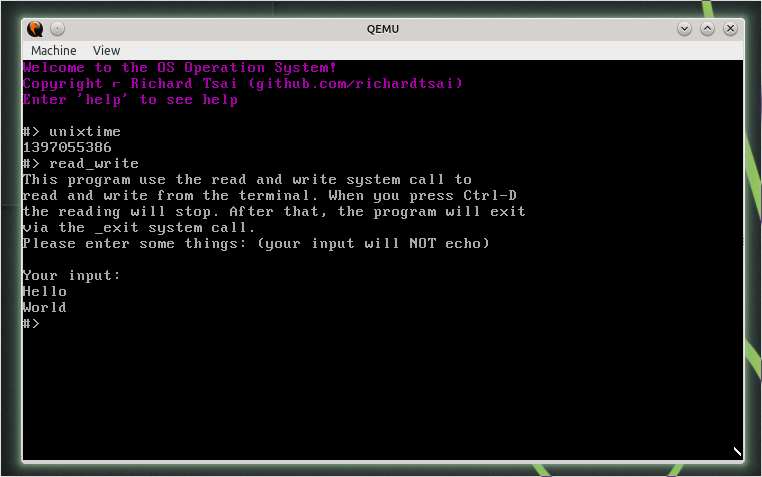
\includegraphics[scale=0.55]{demo.png}

\end{document}
